\section{Clock} \label{sec:clock}
Throughout previous sections, we mentioned a pretty basic term in almost every device of modern technology - (voltage) pulse. In this section, we will answer two questions regarding clocks and corresponding pulses: 

\begin{itemize}
	\item Why do the processor require pulsing? (\ref{sec:clock:why_pulsing})
	\item How do we generate pulses in the processor? (\ref{sec:clock:how})
\end{itemize}

\subsection{Why pulsing?} \label{sec:clock:why_pulsing}
Every digital computer processor, not regarding quantum computing, requires the separation between different cycles, each containing crucial actions such as loading from a register in RAM or performing binary calculations in adders. We achieve such a behavior by biasing an approximate square-wave threshold voltage. It means that at some time intervals, potential difference is 3.3V or, in our case, 5V. At the subsequent interval, the voltage level is grounded. Consequently, at high bias levels operations (or cycles) are being performed whereas low voltage levels are devoid of any action. 
However, most chips nowadays are edge-triggered. It means that the cycles is executed on the edge of pulse where the derivative (dV/dt) is increased or decreased. This behavior is achieved by connecting the voltage square-wave to a filter, rectifier, or some other more primitive techniques. Edge-triggering is indicated on the manufacturer data-sheet.

\subsection{How do we generate pulses?} \label{sec:clock:how}
Firstly, let us state the goal explicitly: we want to have an automatic non-stop square wave, manual-triggered square pulse, and the way to switch between two methods. In our implementation we used a frequently-used chip, the 555 Timer (see \ref{fig:astable}).

Automatic non-stop square wave, or the astable multivibrator, uses the following circuit: 

\begin{figure}[H]
	\centering
	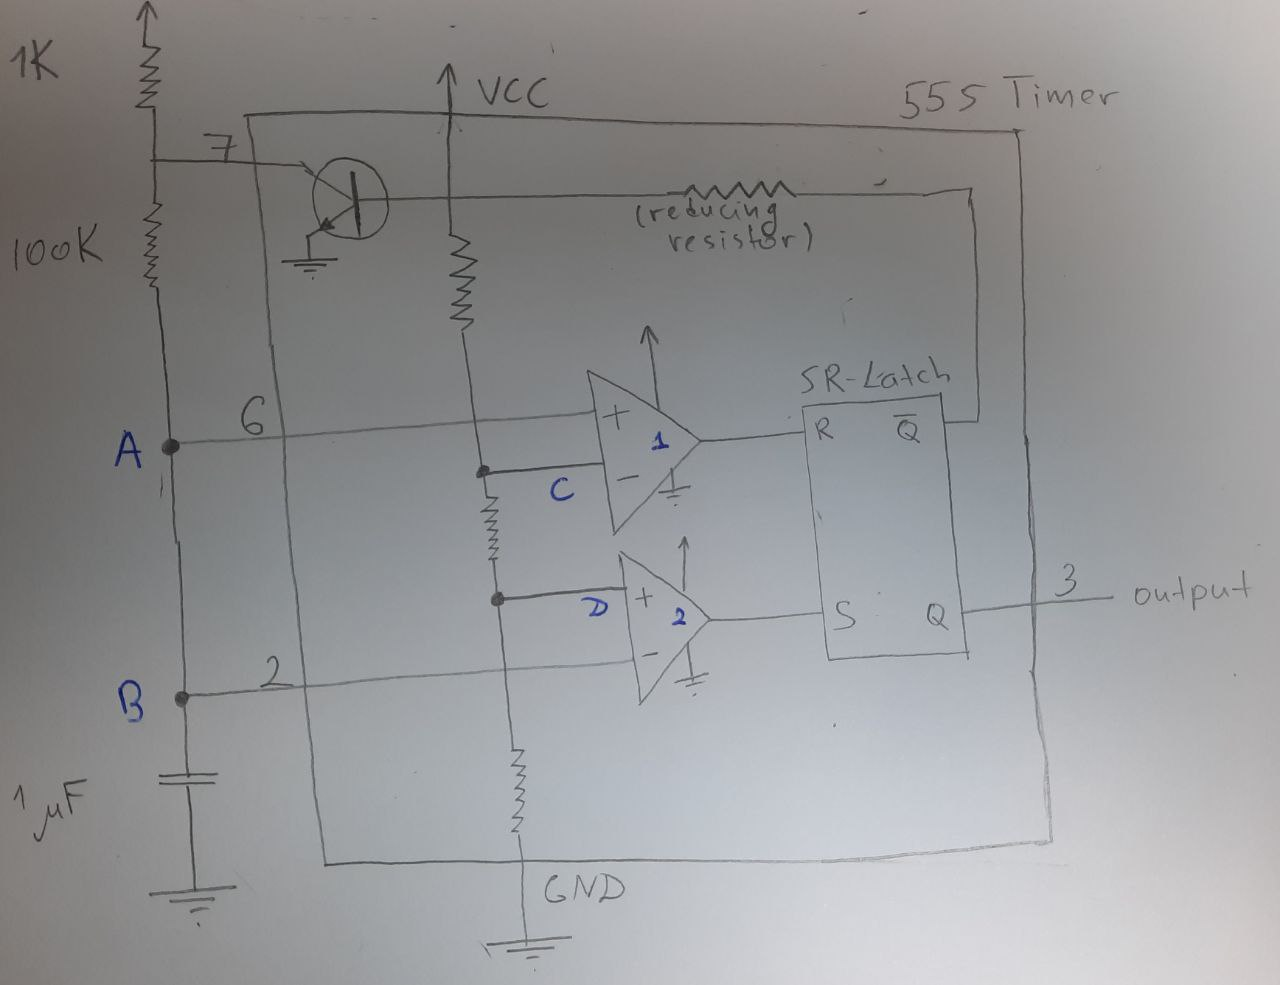
\includegraphics[width=0.7\textwidth]{img/astable}
	\caption{Astable Multivibrator using 555-timer}
	\label{fig:astable}
\end{figure}

The three resistors inside the 555 timer constitute a voltage divider, and configure Op-Amps. The resistors have the same resistance, therefore, if the supplied power is 5V, then point C is at 3.33V whereas the point D is at 1.67V. In the beginning, point A and B\footnote{Note, that they are always at the same potential level, thus we will referring to them simply as A.} are at 0V due to the capacitor. Therefore, only the second Op-Amp outputs voltage (5V), whereas the first one is at 0V. Now, look at the SR-Latch with S set high and R set low. It will make Q high, thus the third pin of the 555 timer is going to be high, which corresponds to the high voltage level of the square wave. During capacitor charging the output is constant. However, when the capacitor is charged enough to set point A at 1.67V, the second operational amplifier turns off, while the first one is not altered. Therefore, S = 0 and R = 0 which means that the output of the 555 is not altered\footnote{The SR-Latch will change the output from High to Low only when R is high.}. The capacitor continues charging and when it has a 3.33V-level, the first Op-Amp is activated. The consequence is that the R of the SR-Latch is high, which makes the output of the 555 timer low, which correspond to the grounded output of the square wave. However, the SR-Latch now outputs voltage to the base of the transistor at pin 7. This makes the collector collect charge and emit it to the ground, thus making two flows to ground: from the voltage supply AND from the capacitor. This action will discharge the capacitor until 1.67V where the SR-Latch will again output high voltage. This is the basic principle of the 555-timer-driven astable multivibrator. The real oscilloscope output is shown in the following figure: 

\begin{figure}[H]
	\centering
	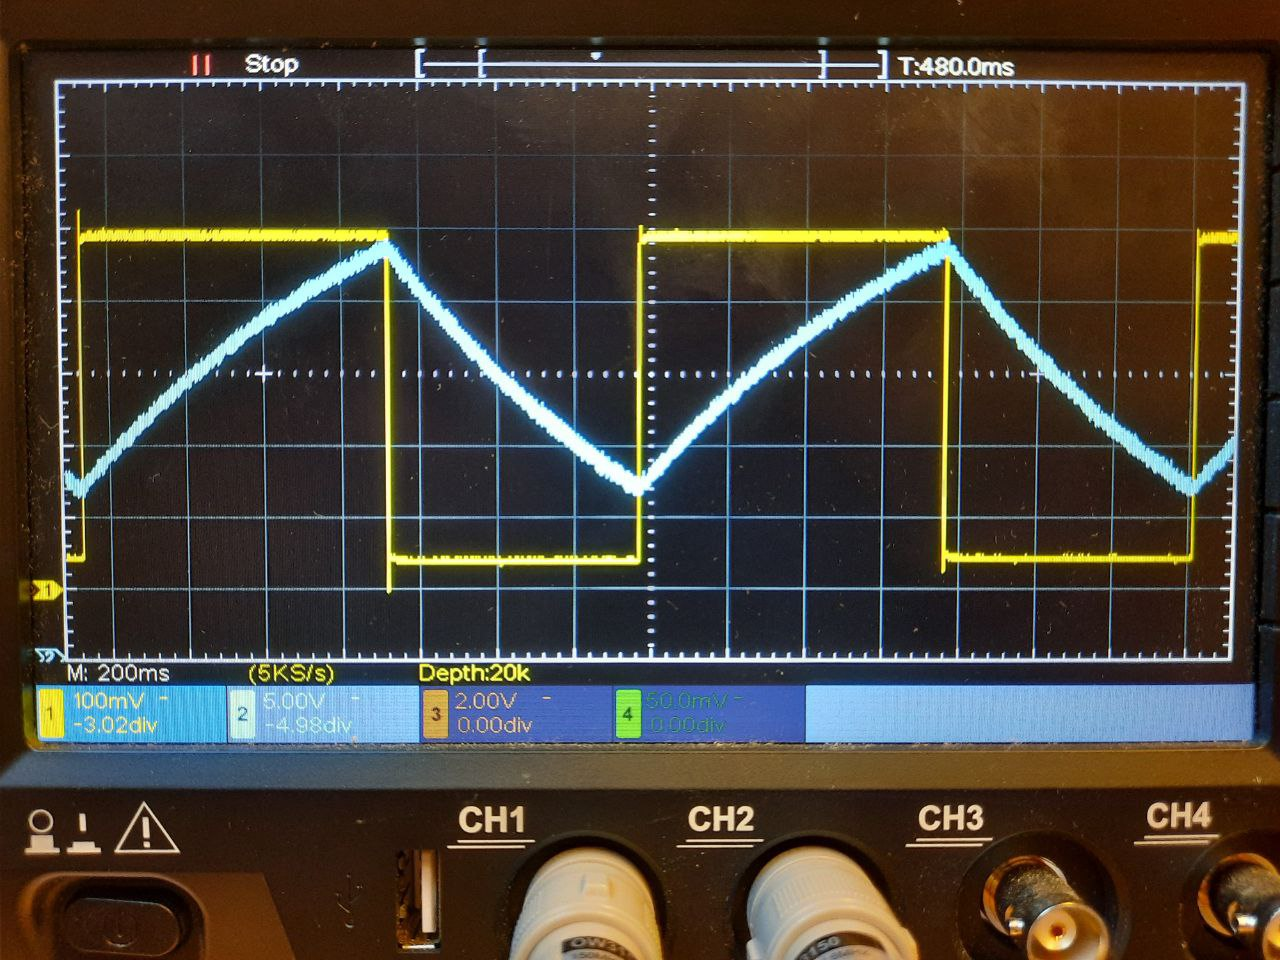
\includegraphics[width=0.9\textwidth]{img/clock_scope}
	\caption{Oscilloscope of the clock and capacitor used with the 555 timer}
	\label{fig:clock_scope}
\end{figure}

Manual-triggered square pulse, or the monostable multivibrator, uses similar principle but voltage to the second pin is supplied only when the button is pressed, see \ref{fig:monostable}. This means that ones pressed, the trigger immediately sets the output high, and keeps it so while being pressed. Once the button is not pressed, the discharging mechanism sets the output low.

\begin{figure}[H]
	\centering
	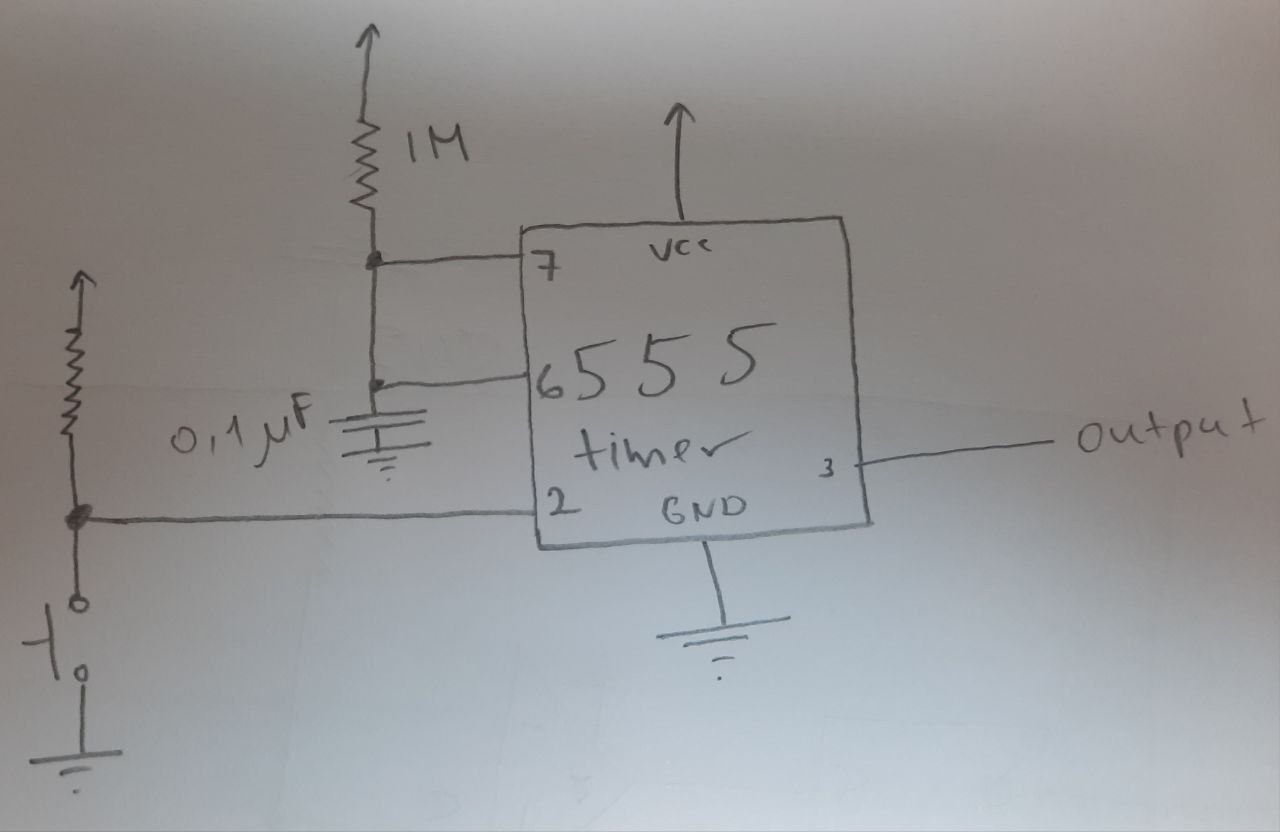
\includegraphics[width=0.9\textwidth]{img/monostable}
	\caption{Monostable Multivibrator using 555-timer}
	\label{fig:monostable}
\end{figure}

The switcher between two modes is implemented by combining several digital gates (NANDs). Further investigation of this part is of no interest and can be traced by looking at the real circuit. The only important thing to note here is that the clock output (so either mono- or astable multivibrator) is ANDed with the hatch pin, which is used for the processor's master reset button. If Hatch is high, the clock is low no matter what is the output of multivibrators.


